\documentclass[../../main.tex]{subfiles}

\graphicspath{{\subfix{../../immagini/}}}

\begin{document}
    Anche per il problema della model selection è possibile sfruttare l'appena introdotta convalida incrociata: l'idea è quella di sfruttare un algoritmo di ottimizzazione per selezionare le varie configurazioni di iperparametri da testare e, per ognuna di queste configurazioni, eseguire una convalida incrociata. La configurazione migliore sarà quella che ottiene un punteggio medio più alto nella cross validation.
    
    In molti casi si vuole però trovare la migliore configurazione di iperparametri e contemporaneamente avere un'idea delle prestazioni del modello, in casi come questo una semplice cross validation non è sufficiente: applicare la convalida incrociata per valutare le prestazione del modello sullo stesso dataset utilizzato per trovare la migliore configurazione di parametri porterebbe infatti a delle stime del modello ottimistiche rispetto alla realtà.

    In contesti come questo si preferisce quindi utilizzare una variante delle cross validation: la convalida incrociata annidata, o nested cross validation. Intuitivamente, questa tecnica consiste nell'annidare due cicli di cross validation: il ciclo più interno è responsabile per la model selection, mentre quello esterno permette di valutare le performance di generalizzazione.

    Più formalmente, la nested cross validation è composta da due cicli annidati con finalità differenti, descritti più del dettaglio di seguito.
    \begin{itemize}
        \item Il ciclo esterno è una normale cross validation: suddivide il dataset in $k$ insiemi di dimensione simile. Ognuno di questi $k$ insiemi viene utilizzato una volta come test set, mentre i rimanenti insiemi compongono il training set. Nel contesto della convalida annidata la peculiarità sta nel modello addestrato: questo infatti avrà una configurazione di iperparametri che corrisponde a quella migliore secondo quanto decretato dal ciclo interno.
        \item Il ciclo interno testa diverse configurazioni di iperparametri tramite una cross validation. In questo caso il dataset su cui la convalida incrociata lavora è il training set del ciclo esterno, e l'insieme che viene usato per il testing prende il nome di validation set.
    \end{itemize}
    In questo modo i $k$ punteggi che vengono restituiti dalla procedura forniscono una stima non distorta delle performance del modello.

    L'algoritmo per la scelta degli iperparametri che utilizziamo negli esperimenti prende il nome di GridSearch: semplicemente dato a priori un insieme di iperparametri, ognuno con un insieme di valori da testare, l'algoritmo testa tutte le possibili combinazioni dei valori di tali iperparametri, decretando poi la migliore.

    Lo svantaggio principale di questa tecnica deriva dalla sua complessità computazionale: in ogni ciclo interno vengono infatti addestrati e valutati $n \cdot k_{in}$ modelli, dove $n$ è il numero di combinazioni di parametri testate e $k_{in}$ è il parametro $k$ della convalida incrociata interna. Questo processo viene poi eseguito per un numero $k_{est}$ di volte, in totale verranno quindi addestrati e testati $k_{est} \cdot n \cdot k_{in}$ modelli.

    La Figura \ref{fig:nestedCV} mostra uno schema del funzionamento della convalida incrociata annidata.

    \begin{figure}[H]
        \centering
        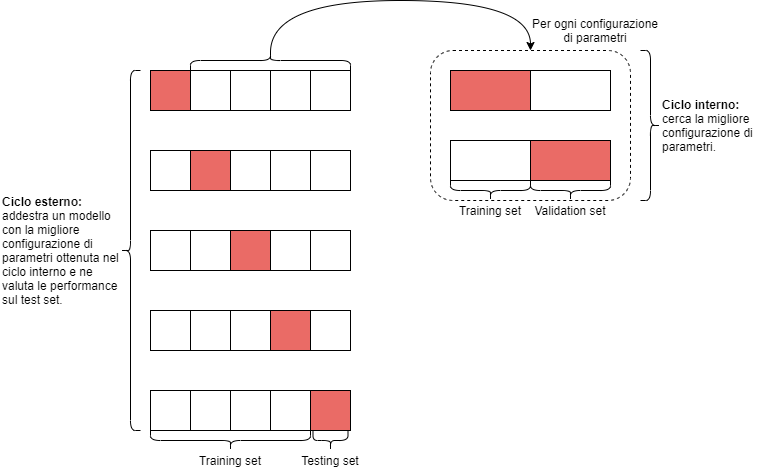
\includegraphics[width=\textwidth]{immagini/6_3/nestedCV.drawio.png}
        \caption{Schema del funzionamento della convalida annidata, in questo caso con $k_{est} = 5$ e $k_{in} = 2$.}
        \label{fig:nestedCV}
    \end{figure}
\end{document}